\documentclass[tikz]{standalone}
\usepackage[dvipsnames,svgnames,x11names]{xcolor}
\usepackage{tikz}
\usepackage{pgfplots}
\pgfplotsset{compat = 1.12}
\usepackage{../thesismath}
\begin{document}
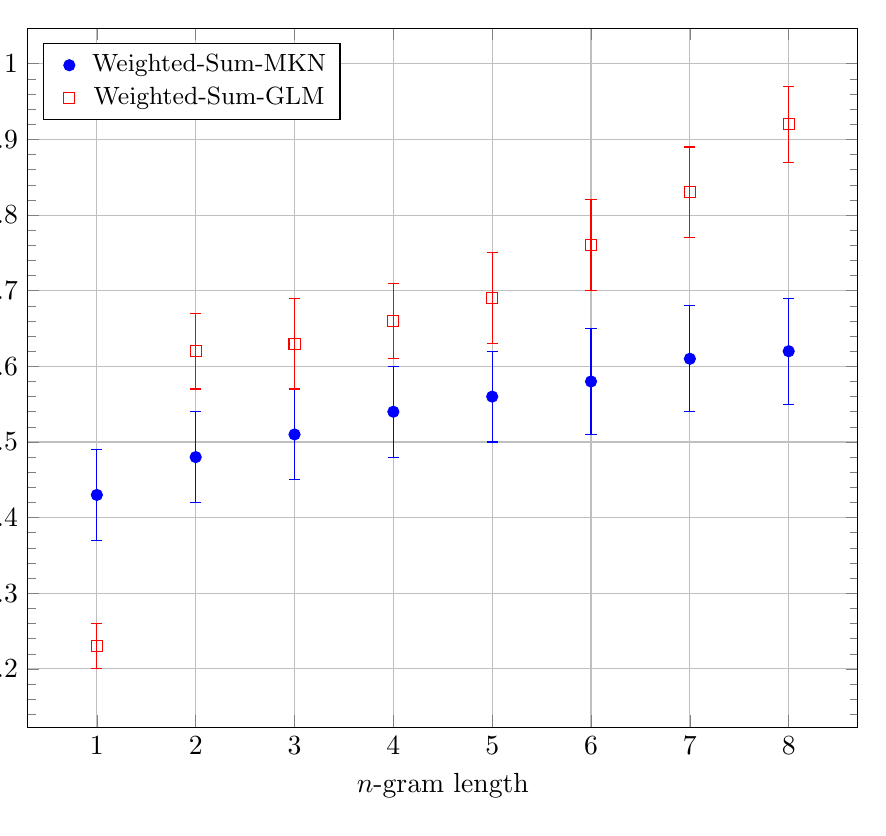
\begin{tikzpicture}[baseline, trim axis left, trim axis right]

\pgfplotscreateplotcyclelist{mkn_glm}{%
  blue,  mark size=2, mark=*,\\%
  red,   mark size=2, mark=square,\\%
}

\pgfplotsset{
  legend style = {
    legend image code/.code = {
      \draw[only marks]
        plot coordinates {
          (0.3cm,0cm)
        };
      \node at (0.15cm, 0cm) {};
      \node at (0.45cm, 0cm) {};
    },
  },
}

\begin{axis}[
%   title = {Relative Weight $\SumWeight^h_i$ Calculation Time per Probability},
  xlabel = {$n$-gram length},
  xtick = {1, ..., 8},
  ylabel = {Relative Calculation Time},
  %ymin = 0,
  minor y tick num = 4,
  grid = major,
  %enlargelimits = 0.025,
  cycle list name = mkn_glm,
  legend entries = {{\small{Weighted-Sum-MKN}}, {\small{Weighted-Sum-GLM}}},
  legend pos = north west,
  legend style = {
    row sep = 0ex,
    xshift = -0.12cm,
    yshift =  0.08cm,
  },
  width = \textwidth,
]

% MKN
\addplot+[
  only marks,
  error bars/.cd,
  y dir = both,
  y explicit,
] table [y error = stddev] {
  n ratio stddev
  1 0.43 0.06
  2 0.48 0.06
  3 0.51 0.06
  4 0.54 0.06
  5 0.56 0.06
  6 0.58 0.07
  7 0.61 0.07
  8 0.62 0.07
%  1 0.79 0.44
%  2 0.95 0.30
%  3 1.08 0.31
%  4 1.22 0.36
%  5 1.34 0.38
%  6 1.48 1.10
%  7 1.62 0.52
%  8 1.75 0.54
};

% GLM
\addplot+[
  only marks,
  error bars/.cd,
  y dir = both,
  y explicit,
] table [y error = stddev] {
  n ratio stddev
  1 0.23 0.03
  2 0.62 0.05
  3 0.63 0.06
  4 0.66 0.05
  5 0.69 0.06
  6 0.76 0.06
  7 0.83 0.06
  8 0.92 0.05
%  1  0.30  0.16
%  2  1.69  1.48
%  3  1.74  0.47
%  4  2.01  1.33
%  5  2.40  0.91
%  6  3.40  1.66
%  7  5.97  6.08
%  8 14.45 16.69
};

\end{axis}

\end{tikzpicture}
\end{document}
